\section{Signalflussdiagramm \formelbuch{213}}
\begin{list}{$\bullet$}{\setlength{\itemsep}{0cm} \setlength{\parsep}{0cm} \setlength{\topsep}{0cm}} 
  \item Graphische Lösung linearer Gleichungen
  \item Graphische Darstellung von LTI-Systemen
  \item Änderung der Topologie ohne UTF zu ändern
\end{list}

\subsection{Glossar \formelbuch{213}}
  \begin{tabular}{|m{4cm} | m{14cm}|}
    \hline
      \textbf{Knoten}: &
      Darstellung einer Grösse, eines Signals oder einer Variable \\
    \hline
      \textbf{Zweig}: &
      Funktionelle Abhängigkeit einer Grösse \\
    \hline
      \textbf{Quelle}: &
      Unabhängiger Knoten, es münden keine Zweige ein \\
    \hline
      \textbf{Senke}: &
      Knoten, ohne weggehende Zweige \\
    \hline
      \textbf{Pfad}: &
      Kontinuierliche Folge von Zweigen, die in die gleiche Richtung zeigen \\
    \hline
      \textbf{Offener Pfade}: &
      Ein Pfad, bei dem jeder beteiligte Knoten nur einmal durchquert wird \\
      \textbf{Vorwärtspfad}: &
      Ein offener Pfad zwischen einer Quelle und einer Senke \\
    \hline
      \textbf{Schleife}: &
      Ein geschlossener Pfad, welcher zum Ausgangsknoten zurückkehrt, 
      wobei jeder beteiligte Knoten nur einmal durchlaufen wird, ausgenommen der
      Ausgangsknoten \\
    \hline
      \textbf{Eigenschleife}: &
      Eine (Rückkopplungs)schleife, die aus einem Zweig und einem Knoten besteht \\
    \hline
      \textbf{Zweigtransmittanz}: &
      Die lineare Grösse, unabhängig von ihrer Dimension, 
      die einen Knoten eines Zweiges zum anderen Knoten in Beziehung setzt. \\
    \hline
      \textbf{Schleifentransmittanz}: &
      Das Produkt der Zweigtransmittanzen in einer Schleife. \\
    \hline
  \end{tabular}

\subsection{Transformationsregeln \formelbuch{219ff.}}
  \begin{multicols}{2}
    \subsubsection{Transmittanzverschiebung\formelbuch{220}}
      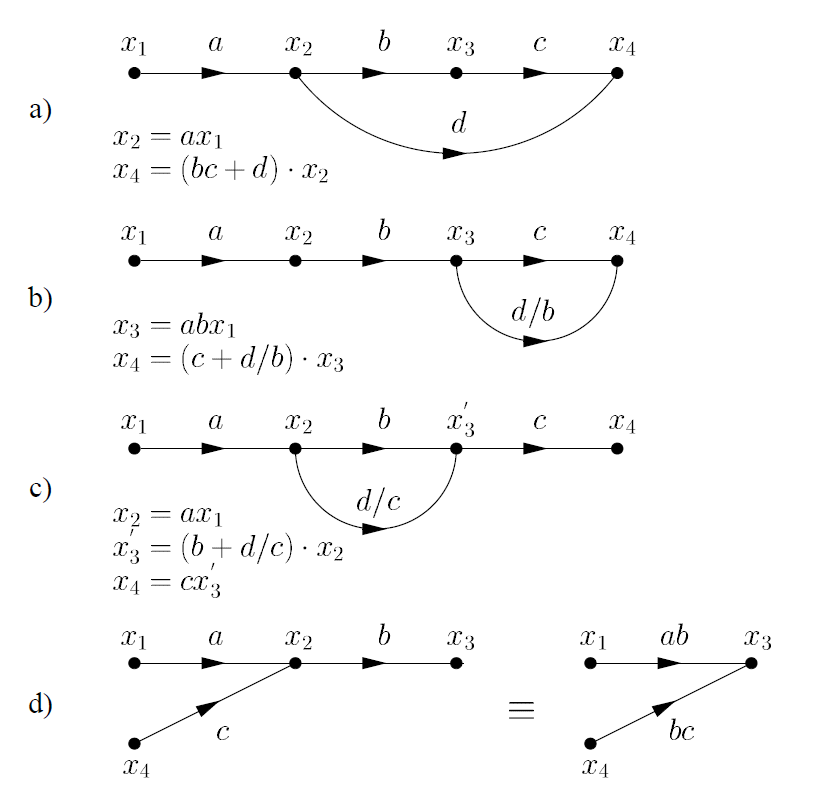
\includegraphics[width=7cm]{./images/transmittanzverschiebung.png} \\
      Wichtig ist, dass eine neue Variable eingeführt wird, wenn wenn der Endpunkt eines
      inneren Zweiges verschoben wird. (siehe c)
      \vfill
  \columnbreak
  
    \subsubsection{Pfadinversion\formelbuch{221}}
      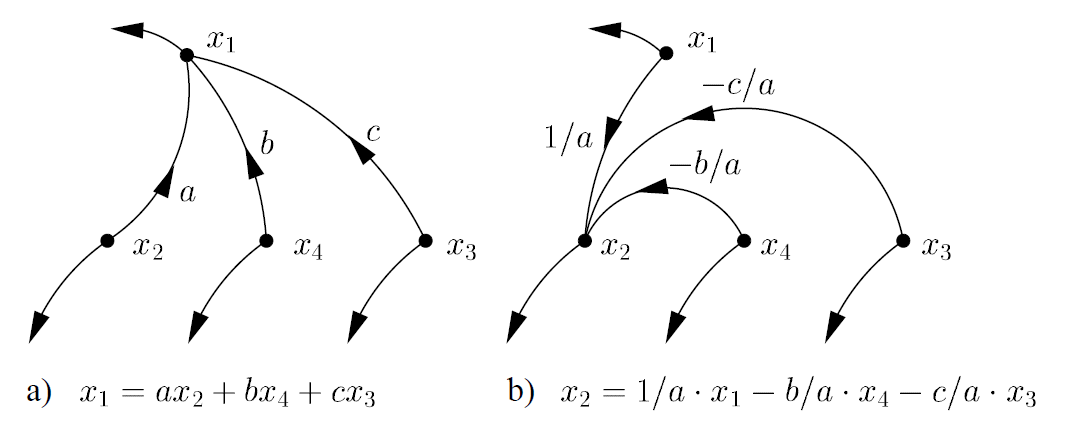
\includegraphics[width=8cm]{./images/pfadinversion.png} \\
      Es gilt zu beachten, das die Inversion eines Pfaden (dessen Anfangspunkt nach Definition
      eine Quelle sein muss) den Effekt hat, dass die Quelle vom einen Ende des Pfades zum anderen
      Ende verschoben wird. Der Pfad von $x_i$ nach $x_j$ hat eine Transmittanz von $L$. 
      Den zu invertierenden Pfad setzten wir $\frac{1}{L}$ und alle Pfade welche ursprünglich in
      $x_i$ endeten, werden verschoben, dass sie neu in $x_j$ enden und ihre Transmittanzen werden
      mit $-\frac{1}{L}$ multipliziert.
      
    \subsubsection{Entfernen einer Eigenschleife\formelbuch{222}}
      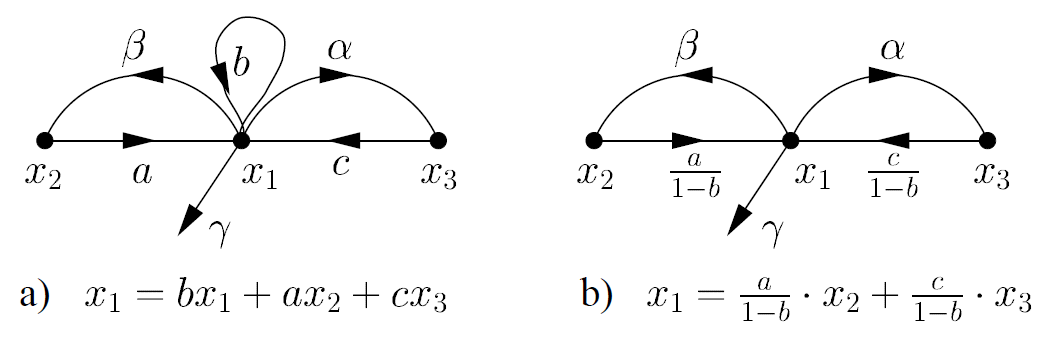
\includegraphics[width=8cm]{./images/eigenschleife.png} \\
      Die Eigenschleife hat die Transmittanz $L$. Sie wird entfernt indem man bei allen anderen
      Zweigen welche \textbf{in den Knoten münden}, durch $(1-L)$ \textbf{dividiert}.
 \end{multicols}
 
\newpage 

\subsection{Mason's Regel \formelbuch{227}}
  $\boxed{H_{ij} = \frac{\sum\limits_k P_k\cdot\Delta_k}{\Delta}}\quad
  \Rightarrow$ UTF von $x_i$ nach $x_j$, wobei \textbf{$x_i$} eine
  \textbf{Quelle}, \textbf{$x_j$} jedoch nicht zwingend eine \textbf{Senke} sein
  muss. \vspace{0.3cm}\\
  $P_k \Rightarrow$ Vorwärtspfad $k$ (bezogen auf 1 Eingang) \qquad $\Delta_k \Rightarrow$ Kofaktor de
  $k$-ten Pfades \qquad $\Delta \Rightarrow$ Netzwerkdet/Graphdet\vspace{0.3cm}\\
  $\Delta$ = 1- (Summe aller Schleifen) + (Summe aller Produkte zweier
  Schleifen, die sich nicht berühren) - (Summe
  aller Produkte dreier Schleifen, die sich nicht berühren) + $\ldots$
  \vspace{0.3cm}\\
  $\Delta_k$ = 1- (Summe aller Schleifen die $P_k$ nicht berühren) + (Summe
  aller Produkte zweier Schleifen, die $P_k$ und sich selbst nicht
  berühren)-(Summe aller Produkte dreier Schleifen, die $P_k$ und sich selbst
  nicht berühren) + $\ldots$ \\

  Falls die \textbf{UTF eines SFD von einem beliebigen Knoten} (keiner Quelle)
  gesucht wird, kann Mason's Regel nicht direkt angewandt werden. Abhilfe: \\
  $\boxed{H_{ij} = \frac{x_j}{x_i} = \frac{x_j}{x_q} \frac{x_q}{x_i} =
  \frac{H_{qj}}{H_{qi}}}$ Wobei $x_q$ eine Quelle sei. 
  Schlussendlich kürzt sich die Netzwerkdeterminante heraus.


\subsection{Beispiel eines SFD \formelbuch{231}}
\begin{tabular}{ll}
	\parbox{7cm}{
    	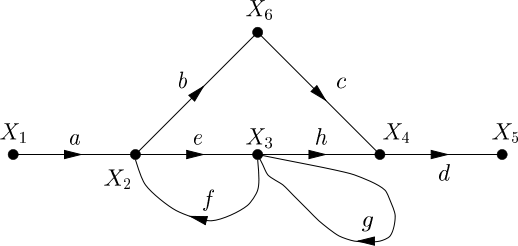
\includegraphics[width=7cm]{./images/sfd-bsp.png}
    }
    
    & \parbox{12cm}{
    \begin{enumerate}
		\item[a)] Die UTF\index{UTF} zwischen $X_1$ und $X_4$ ist (mit Mason's Regel):\index{Mason's Regel}\\
		\begin{equation*}
		H_{14}=\frac{X_4}{X_1}=\frac{aeh+abc(1-g)}{1-ef-g}
		\end{equation*}
		\item[b)] Das folgende Gleichungssystem beschreibt das SFD.
		\begin{eqnarray*}
		X_2 &=&a\cdot X_1+f\cdot X_3\\
		X_3 &=&e\cdot X_2+g\cdot X_3\\
		X_4 &=&h\cdot X_3+c\cdot X_6\\
		X_5 &=&d\cdot X_4\\
		X_6 &=&b\cdot X_2
		\end{eqnarray*}
		Nach Umformung der Gleichungen erhalten wir:
		\begin{equation*}
		X_4=h\cdot X_3+\frac{bc}{e}\cdot (1-g)\cdot X_3\quad\&\quad X_3\cdot
		\frac{1-g}{e}=a\cdot X_1+f\cdot X3.
		\end{equation*}
		Somit ist $X_4=\frac{h+\frac{bc}{e}(1-g)}{\frac{1-g}{ae}-\frac{f}{a}}X_1=\frac{aeh+abc(1-g)}{1-g-ef}X_1$.
	\end{enumerate}}
\end{tabular}

\subsection{Fundamentales SFD \formelbuch{232}}
\begin{tabular}{ll}
	\parbox{7cm}{
    	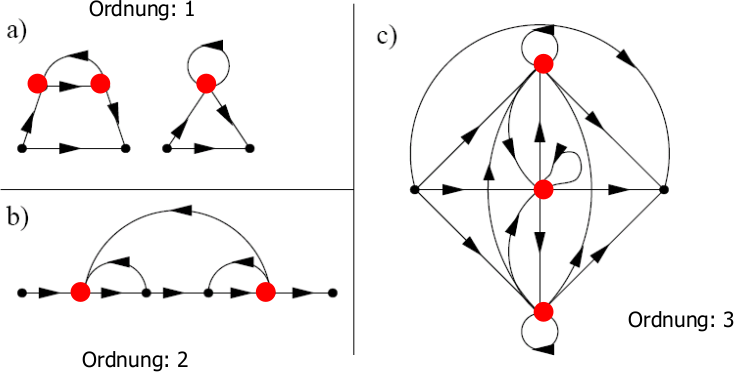
\includegraphics[width=7cm]{./images/sfd-ordnung.png}
    }
    
    & \parbox{12cm}{
		\textit{Ordnung eines SFD = Anzahl der fundamentalen Knoten}: Knoten, welche
		entfernt werden müssen, um \textit{alle} Schleifen aufzubrechen. \\ \\
	}
\end{tabular}

\subsubsection{Fundamentales SFD erster Ordnung \formelbuch{233}}
\begin{tabular}{ll}
	\parbox{7cm}{
    	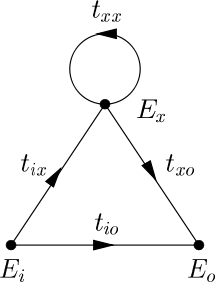
\includegraphics[width=3cm]{./images/sfd-fundamental-erster-ordnung.png}
    }
    & \parbox{12cm}{
		Durch Reduzieren auf das fundamentale SFD 1. Ordnung, kann die UTF direkt
		ermittelt werden: \\
		\[ H_{io} = \frac{E_o}{E_i}=
		t_{io}+\frac{t_{ix}t_{xo}}{1-t_{xx}}=
		\frac{t_{io}-t_{io}t_{xx}+t_{ix}t_{xo}}{1-t_{xx}} \] \\
    \begin{tabular}{l l p{8cm}}
      $E_x$ & = & Fundamentaler Knoten\\
      $E_i$ & = & Quelle (Eingang) \\
      $E_o$ & = & Senke (Ausgang) \\
      $t_{xx}$ & = & alle Eigenschleifen des Knoten $E_x$ \\
      $t_{ix}$ & = & alle Pfade von der Quelle zum Knoten $E_x$ \\
      $t_{xo}$ & = &alle Pfade vom Knoten $E_x$ zur Senke \\
      $t_{io}$ & = & Leckpfad, alle Pfade von der Quelle zur Senke, welche \underline{nicht}
      durch den Knoten $E_x$ führen.
    \end{tabular}\\
    Wenn es mehrere Wege gibt, dann zusammen zählen: Bsp.: $tix = tix_1 +
    tix_2$
	}
\end{tabular}


\subsection{Einbezug analoger Verstärker \formelbuch{238}}
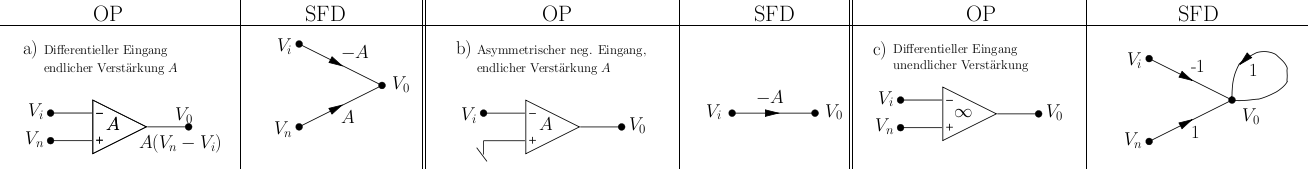
\includegraphics[width=18cm]{./images/sfd-op.png}

\subsection{Skalierung\formelbuch{243}}
	Um einen oder mehrere Knoten zu ändern, ohne das gesamte System zu
	ändern (Voraussetzung: Start/Endknoten werden nicht mitmaskiert), kann man
	diese Knoten skalieren.\\
	Vorgehen: 
	\begin{enumerate}
                \item Skalierungszone festlegen (Trennbündel) $N_b$
                \item Alle eingehende Zweige mit $\lambda$ multiplizieren
                \item Alle ausgehende Zweige mit $\frac{1}{\lambda}$
                multiplizieren
    \end{enumerate}
    Wenn alle maximalen Signalniveaus gleich $\rightarrow$ maximal möglichen
    Dynamikbereich\\
    \begin{minipage}{9cm}
      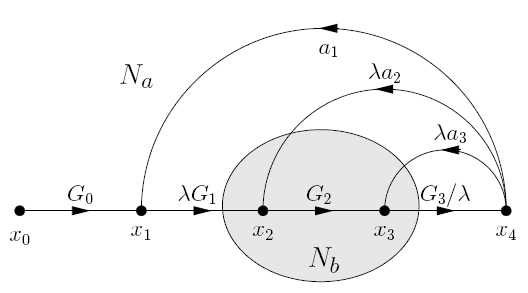
\includegraphics[width=7cm]{./images/sfd-scalierung.png}
    \end{minipage}
    \begin{minipage}{9cm}
      Die Skalierung kann verwendet werden um den Dynamikbereich zu maximieren, Inverter zu entfernen
      und die Verstärkung und Signalniveaus innerhalb eines Systems zu ändern.
    \end{minipage}
    
\subsection{Transposition\formelbuch{242}}
  \begin{multicols}{2}
    \textbf{Ablauf:}
    \begin{enumerate}
      \item Richtungsumdrehung aller Zweigtransmittanzen bei gleichbleibenden Transmittanzen
      \item Spiegelung des resultierenden SFD
      \item Bezeichnungswechsel von Eingangs- und Ausgangsknoten
    \end{enumerate}
    
    Die UTF des transponierten SFD ist \textbf{identisch} mit der UTF des ursprünglichen SFD, aber ihre
    Topologie ist verschieden.
    
  \columnbreak
    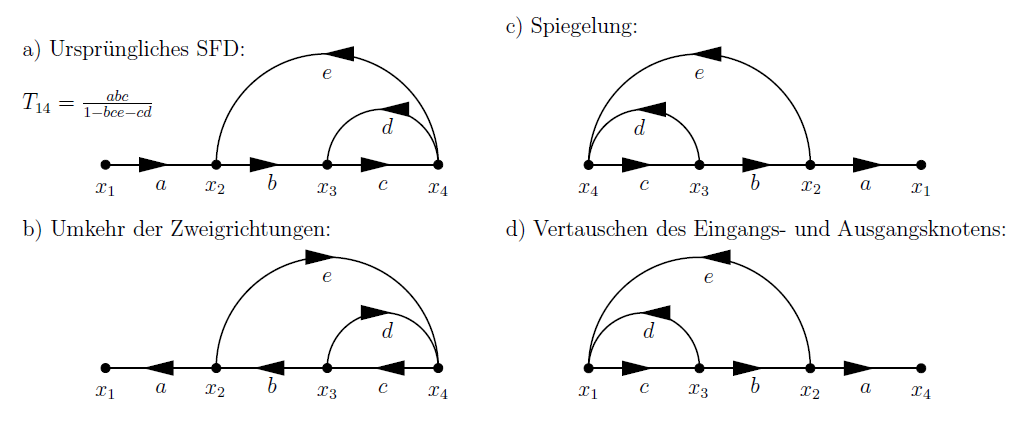
\includegraphics[width=9cm]{./images/transposition.png}
  \end{multicols}
    

